\newpage
\chapter{Design} 

\section{Convolutional Neural Network}
    \subsection{CNN Model Architecture}
    \noindent
    One of the most popularly used CNN model architectures is the VGG19 (Visual Geometry Group) architecture. It consists of 19 weight layers comprising 16 convolutional layers and 3 fully connected layers. The key components of the VGG19 architecture are:
    \begin{enumerate}
        \item Convolutional Layers: 3x3 filters with a stride of 1 and padding of 1.
        \item Activation function: ReLU (Rectified Linear Unit) applied after each convolutional layer.
        \item Pooling layers: Maxpooling layers with a 2x2 filter and a stride of 2.
        \item Fully connected layers: Three fully connected layers at the end of the network, at the end of classification.
        \item Softmax Layer: Final layer for classification with probabilities.
    \end{enumerate}
    The architecture of the CNN model consists of multiple key layers, including convolutional layers, pooling layers, and dense (fully connected) layers. The convolutional layer is responsible for feature extraction, utilising the Rectified Linear Unit (ReLU) activation function to introduce non-linearity and enhance the learning of complex patterns. To reduce the spatial dimensions and computational complexity while retaining the most essential features, max pooling is applied. This operation selects the maximum value from a defined window, preserving crucial information. Following the convolutional and pooling layers, a flattening layer is used to convert the multi-dimensional feature maps into a one-dimensional vector, which is then passed to the dense layer. The dense layer is fully connected, meaning each neuron in one layer is linked to every neuron in the next layer. This layer utilises the softmax activation function for classification, enabling the model to output probability distributions corresponding to benign or malignant categories. \par \noindent
    The CNN model is implemented using Python with the TensorFlow machine learning framework, which provides a comprehensive set of tools for designing, training, and optimising deep learning models. TensorFlow’s flexibility and efficiency allow for the seamless deployment of CNN-based solutions for real-time decision-making in thyroid nodule classification.

    \begin{figure}[ht]
        \centering
        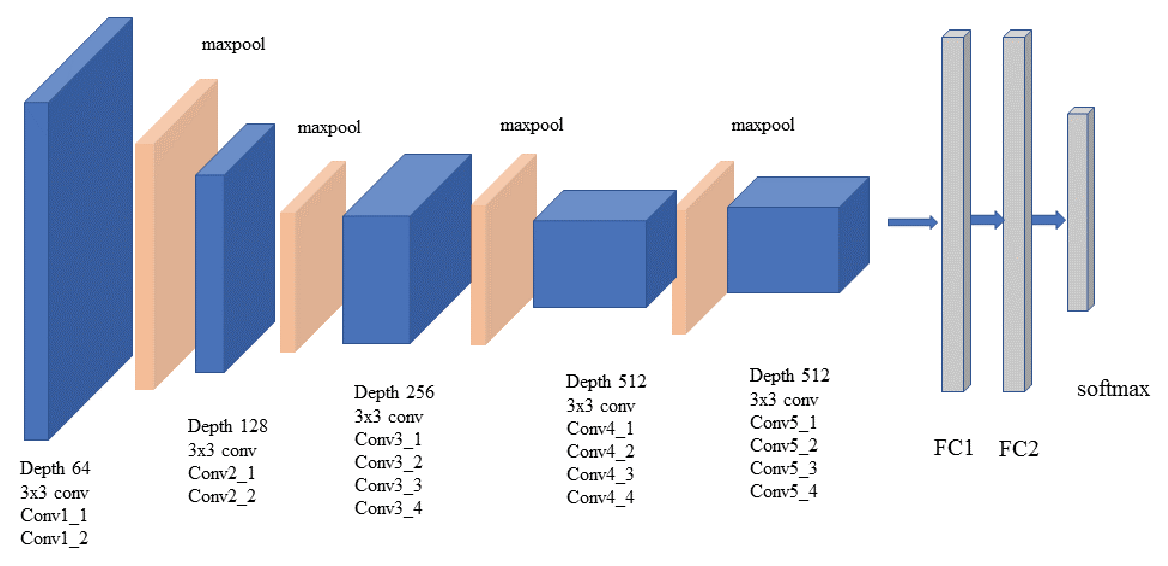
\includegraphics[width=0.75\linewidth]{images/vgg19.png}
        \caption{The VGG19 model architecture}
        \label{fig:vgg19}
    \end{figure}

    \subsection{CNN FPGA Deployment}
    \noindent
    As the number of layers increases, the model requires more compute resources, and the FPGA used, i.e. PYNQ Z2, has a limited number of resources. Thus, it may not be possible to deploy a large model, along with the fact that the design, development and testing of the implementation at the FPGA level is a very time-consuming task. Hence, for the sake of simplicity and considering the above points, this project uses a simple 3-layer Convolutional Neural Network Architecture consisting of a Convolutional layer, Maxpool layer and a dense layer for FPGA Deployment, and at each stage \textit{relu} is used as an activation function. The model summary of the model being considered for deployment is shown in figure \ref{fig:model_summary}. Figure  \ref{fig:CNNpartition} briefly illustrates the partitioning of the CNN model acceleration scheme for the model under consideration. Along with other partitioned tasks being employed in the partitioning scheme.

    \begin{figure}
        \centering
        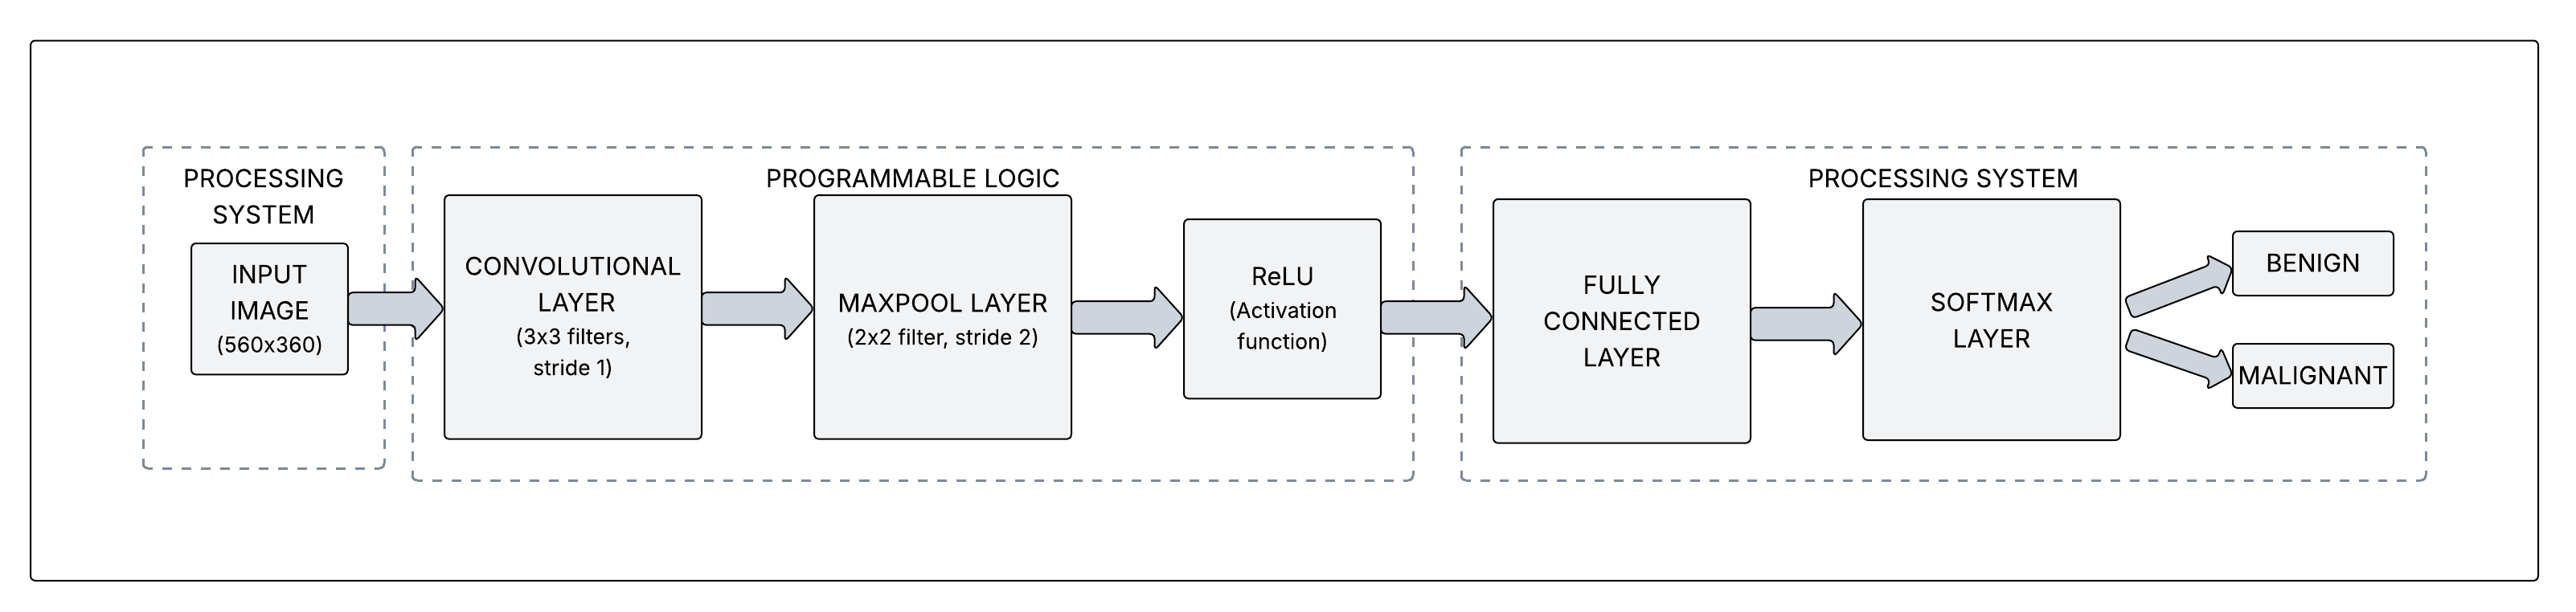
\includegraphics[width=1\linewidth]{images/newCNNdiag.png}
        \caption{CNN Model and Partitioning scheme}
        \label{fig:CNNpartition}
    \end{figure}
    
    \begin{figure}[H]
    \centering
    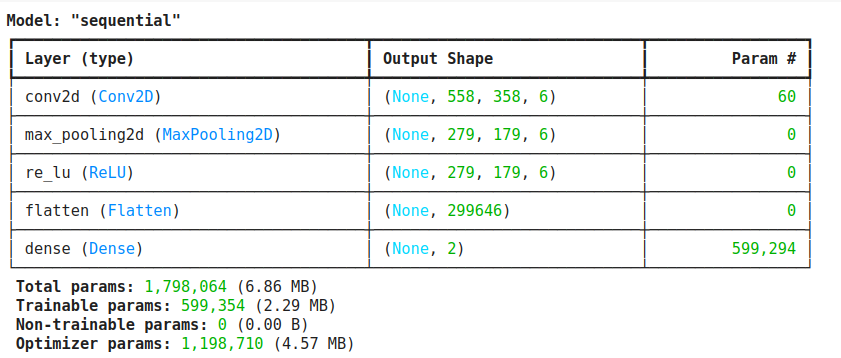
\includegraphics[width=\textwidth]{images/model_summary.png}
    \caption{Model Summary Table}
    \label{fig:model_summary}
    \end{figure}

    \section{Processing System}
    \noindent
    The processing system (PS) refers to the processor on the PYNQ Z2, which is an ARM Cortex A9 dual-core processor. As mentioned earlier, this is used for implementing the fully connected layer. The PS, apart from computing the result from the fully connected layer, is also responsible for receiving the input image for classification through the UART interface and then transferring it to the PL using the DMA. The top module collects data from the DMA, which transfers the data through the AXI MM2S interface, which is shown in Figure \ref{fig:overall_block}.

    \begin{figure}[H]
    \centering
    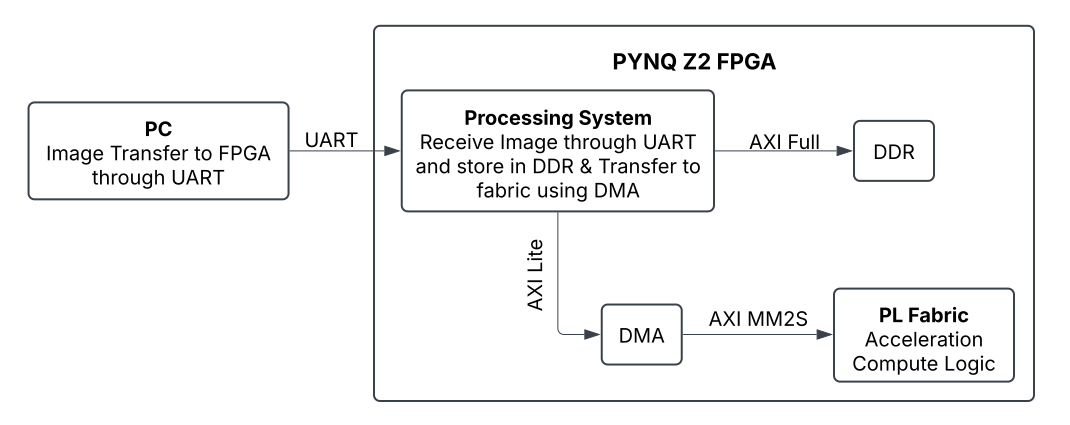
\includegraphics[width=\textwidth]{images/OverallBlockDiagram.png}
    \caption{Overall high-level view of FPGA acceleration scheme}
    \label{fig:overall_block}
    \end{figure}

    \section{AXI Protocol}
    \noindent
    The AXI protocol is widely used across the system design of the entire project. The AXI protocol comes in three variants: 
    \begin{enumerate}
    % \setlength{\itemsep}{0.5pt}
    % \setlength{\parskip}{0.5pt}
    % \setlength{\topsep}{0.5pt}
    \item AXI Full
    \item AXI Lite
    \item AXI Stream
    \end{enumerate}
    \noindent
    Out of which the first two are memory-mapped interfaces, while AXI Stream is not, making it a simpler one among the three to implement and reducing memory overhead, thus the acceleration logic deployed on the fabric uses an AXI Stream protocol. The DDR, being a memory-mapped peripheral, communicates with the PS using the AXI Full protocol, whereas DMA, which is also a memory-mapped interface, communicates with the PS through the AXI Lite interface. Now that our PL logic is based on the AXIS protocol, the DMA, which consists of bridging logic, communicates with PL through AXI MM2S (memory-mapped to stream) interface. Figure \ref{fig:AXI_Stream_block} shows a simple interface between two AXI Stream peripherals, with ready, valid and data signals, apart from the clock and reset, other signals are optional and hence not shown. Figure \ref{fig:axi_stream_waveform} shows AXIS protocol waveforms, only the ready, valid and data signals are taken in our implementation, as the rest of the signals are optional.

    \begin{figure}
        \centering
        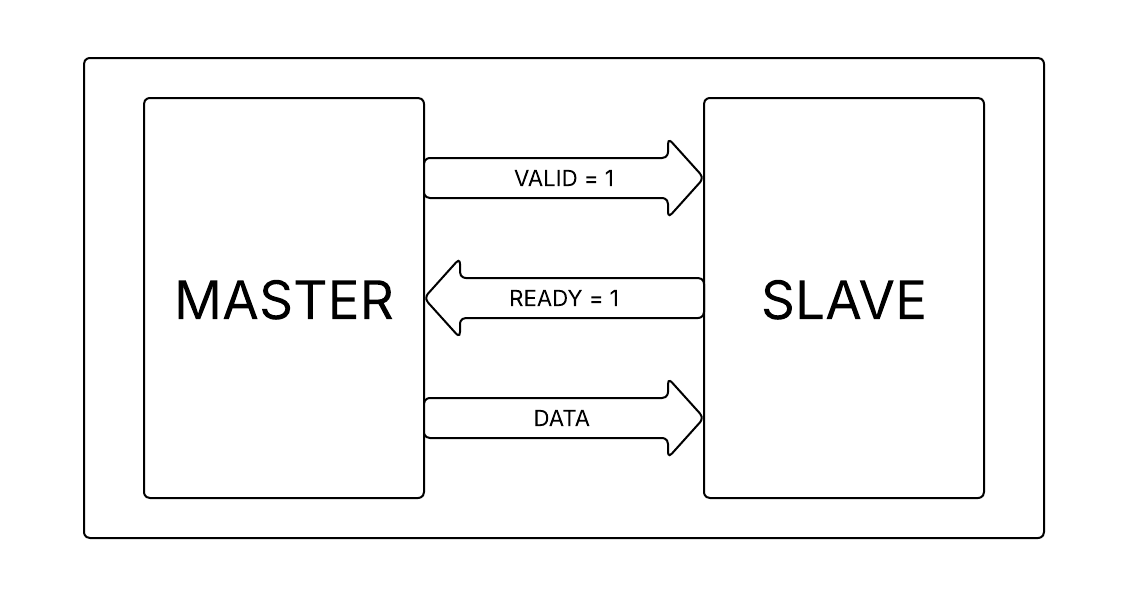
\includegraphics[width=0.75\textwidth]{images/axi_image.png}
        \caption{AXI Stream block interface}
        \label{fig:AXI_Stream_block}
    \end{figure}

    
    \begin{figure}[H]
    \centering
    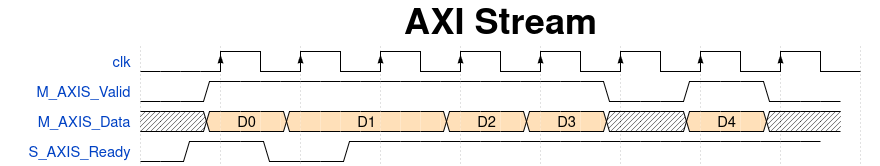
\includegraphics[width=\textwidth]{images/AXI_StreamWaveDrom.png}
    \caption{AXI Stream Protocol Waveform}
    \label{fig:axi_stream_waveform}
    \end{figure}

    \section{PL Fabric}
    \subsection{Data Representation}
    \noindent
    The CNN model when designed on PC uses float32 format to store the weights and biases which are associated with the convolutional and fully connected layer but using float representation on FPGA would be very expensive considering the amount of available resources for logic implementation so a fixed point scheme is adopted instead where MSB represents the sign bit and following three bits represent integer part and remaining bits represent the fraction bits. The integer bits are 3 bits wide because the weights and biases are not larger than the possible range of representation. Further, after certain computations such as multiplication or addition, the integer width is adjusted to accommodate the result adequately without loss of significant bits. Figure \ref{fig:fixed_point} shows the fixed point representation, width and bit position.

    \begin{figure}[ht]
    \centering
    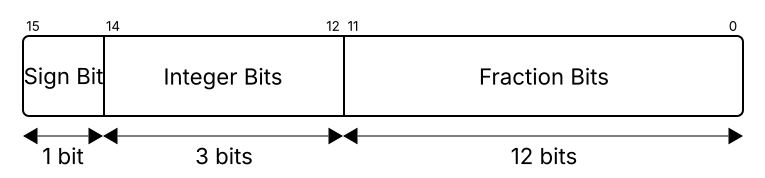
\includegraphics[width=\linewidth]{images/Data_16Bit_Representation.png}
    \caption{Data Representation for Weight \& Biases}
    \label{fig:fixed_point}
    \end{figure}

    \subsection{Convolution Layer Architecture} \label{sec:conv_architecture}
    \noindent

    \begin{figure}[H]
        \centering
        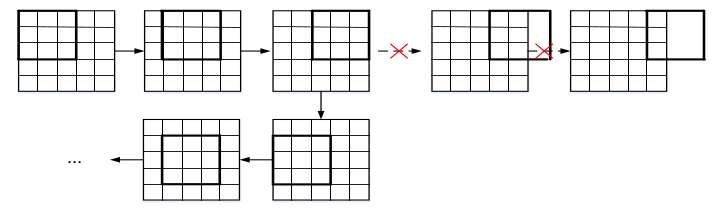
\includegraphics[width=\textwidth]{images/conv_window.png}
        \caption{Convolution operation window}
        \label{fig:conv_window}
    \end{figure}

    \noindent Figure \ref{fig:conv_window} shows how the filter moves across the image in a convolution operation, and is modelled to operate the same way at the hardware level.
    The convolutional layer uses 4 line buffers to store the data required for the convolution operation as shown in figure \ref{fig:line_buffer_architecture}, one line buffer stores data from one row of the image, since the kernel is a 3x3 kernel at least 3 line buffers are required for the operation, while 3 line buffers are being read one line buffer is storing data from the PS. The 4-line buffer structure takes one pixel of image data at every clock edge. The three-line buffers, which are being read, give data of 3x3, i.e. 9-pixel values, 8 bits wide, which is 72 bits wide. The modelling of the convolution operation is discussed in more detail in the subsequent section, as the data and control logic, as a whole, the convolution operation is wrapped in a top module comprising both data and control logic.
    
    

    \begin{figure}[H]
    \centering
    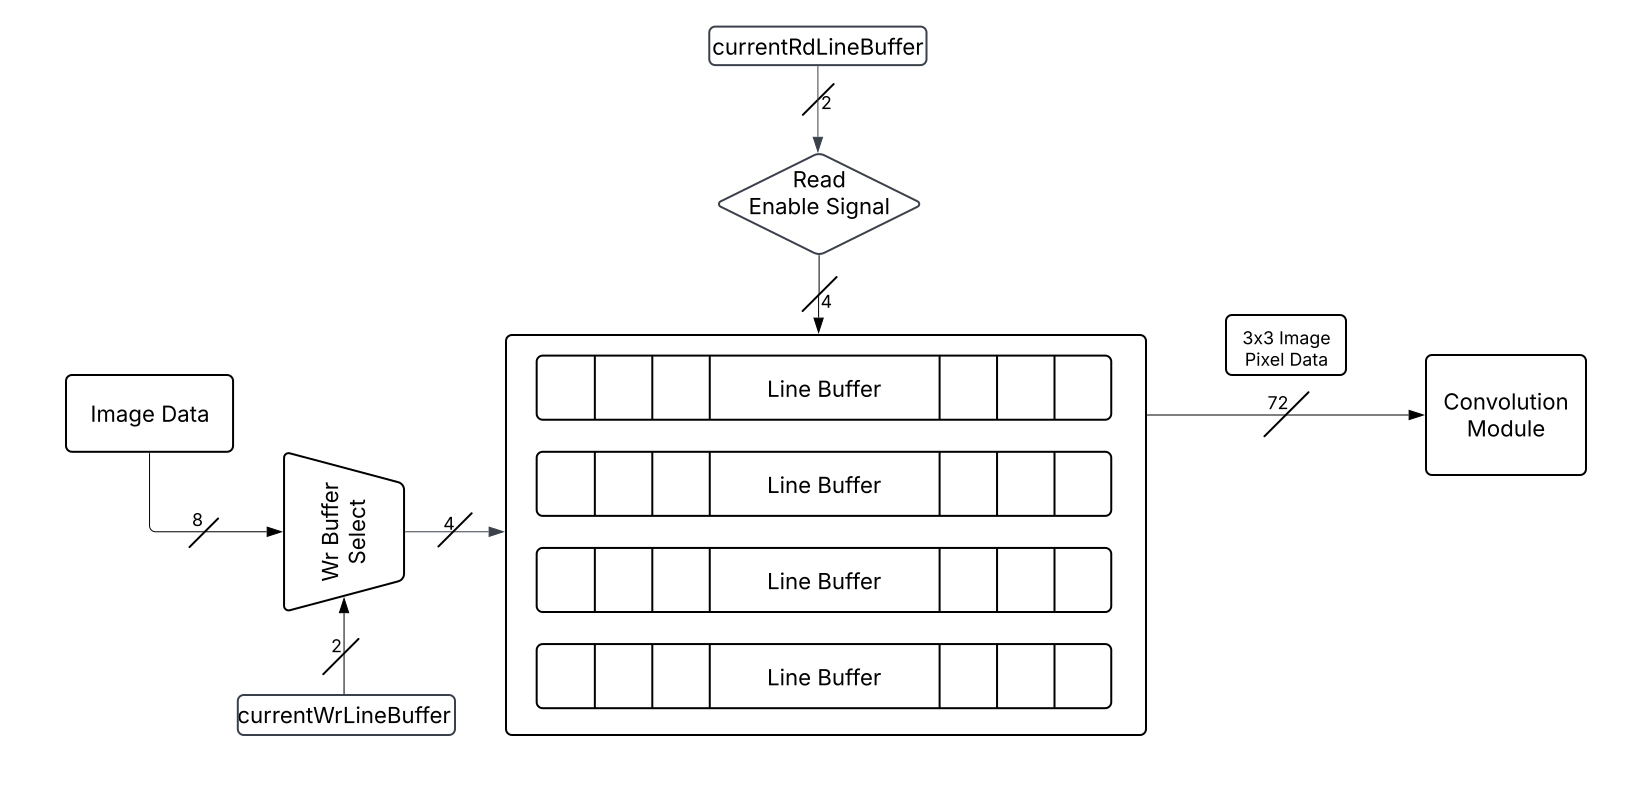
\includegraphics[width=\linewidth]{images/CONV_Architecture.png} 
    \caption{Convolution Layer line buffer architecture}
    \label{fig:line_buffer_architecture}
    \end{figure}

    \noindent
    \subsubsection{Data Logic}
    \noindent
    The convolution module upon receiving the data from line buffers computes the result for one set of 3x3 pixels in 4 stages which are shown in figure \ref{fig:pipeline_architecture}, in the first stage all the data is multiplied in a parallel fashion and stored in 9 registers(0-9) shown in figure \ref{fig:pipeline_architecture} in the second stage, these are added 3 at a time and their results are stored in 3 registers(Sum1, Sum2 \& Sum3) shown in the figure \ref{fig:pipeline_architecture} this addition occurs as soon as the multiplication results are available that is achieved because this stage is modelled in a combinational manner to reduce one clock latency, the next stage sums the data in those 3 registers to generate the convolution result, the fourth stage performs \textit{relu} operation which is an activation function and adds the bias to the result of convolution. The stagewise completion of the convolution operation is indicated by the \textit{valid} signal, which propagates through stages, the \textit{valid} signal going high at the final stage means the convolution operation result is available. The result of the convolution is 24 bits wide, MSB as the sign bit followed by 11 bits of integer part and remaining bits to represent fraction part, is shown in figure \ref{fig:conv_result}.

    \noindent The equation given below shows the \textit{relu} operation.

    \[
    f(x) =
    \begin{cases} 
    x & \text{;  } x > 0 \\
    0 & \text{;  } x \leq 0
    \end{cases}
    \]

    \begin{figure}[H]
    \centering
    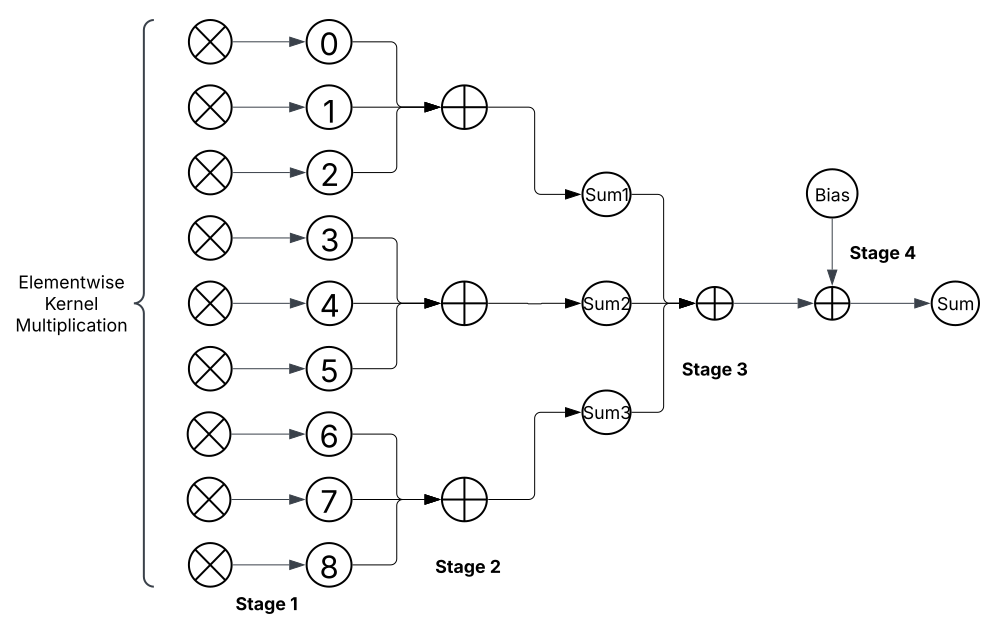
\includegraphics[width=\linewidth]{images/MAC_Unit.png} 
    \caption{The Convolution operation stagewise implementation scheme}
    \label{fig:pipeline_architecture}
    \end{figure}

    \begin{figure}[H]
        \centering
        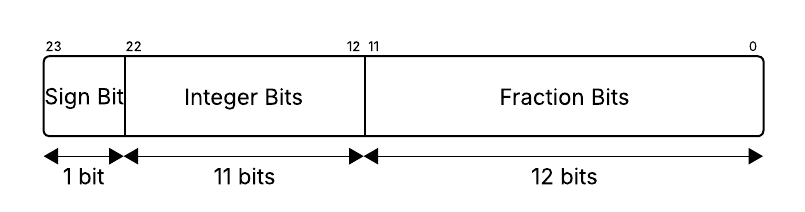
\includegraphics[width=\textwidth]{images/conv_result.png}
        \caption{Convolution result width format}
        \label{fig:conv_result}
    \end{figure}

    \subsubsection{Control Logic}
    \noindent
    One point to note in convolution operation is inorder to compute convoluted result 3 rows of data i.e. 3 line buffers must be ready with the data, figure \ref{fig:threeLineBuffcontrol} shows the state diagram for the same, the totalPixelCounter counts whether three line buffers have been filled or not by monitoring the input valid signal \textit{i\_data\_valid} while data is not being read, totalPixelCounter as shown in figure does not update its count while read and write occur simultaneously since it means one pixel is being written and one is being read so total pixel count does not change, while no data is being read totalPixelCounter decrements. 

    \begin{figure}[H]
    \centering
    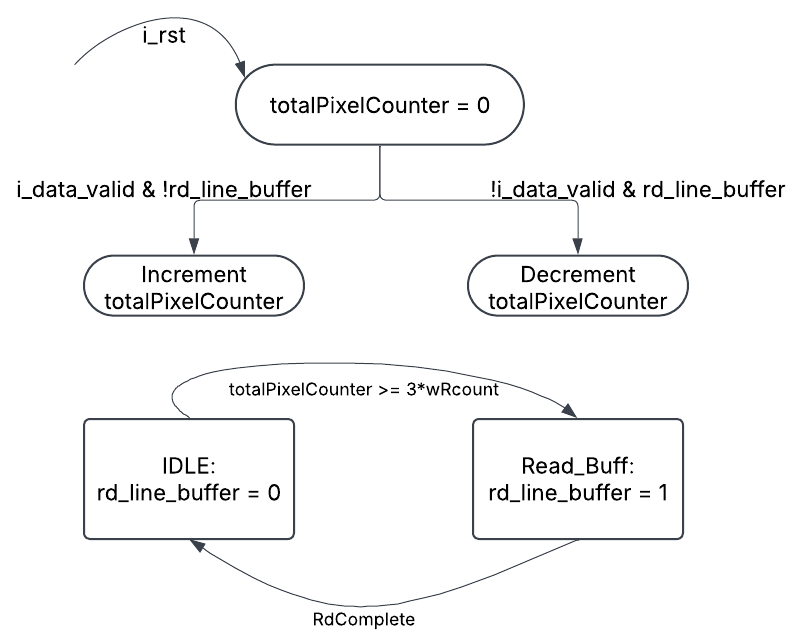
\includegraphics[width=0.75\linewidth]{images/readTotalCount.png}
    \caption{Control logic for read signal}
    \label{fig:threeLineBuffcontrol}
    \end{figure}

    \noindent
    The convolution operation involves shifting the kernel, which is handled by the control logic. The ‘currentWrlinebuffer’, ‘currentRdlinebuffer’ keep a track of which buffer to write new data and which buffers to read from. Figure \ref{fig:wrBufferControl} and \ref{fig:rDBufferControl} represent the counter and state diagram used to generate ‘currentWrlinebuffer’ and ‘currentRdlinebuffer’ signals.
    Here, wRcounter and Rdcounter have a similar task they go high whenever writing and reading, respectively, of a row is completed. These signals keep updating the ‘currentRdlinebuffer’ and ‘currentWrlinebuffer’, and the state of these two signals generates read and write \textit{valid} or, in simple words, enable signals. The reading operation reads three line buffers at a time in a cyclic fashion, while the write operation writes to one line buffer.

    \begin{figure}[H]
    \centering
    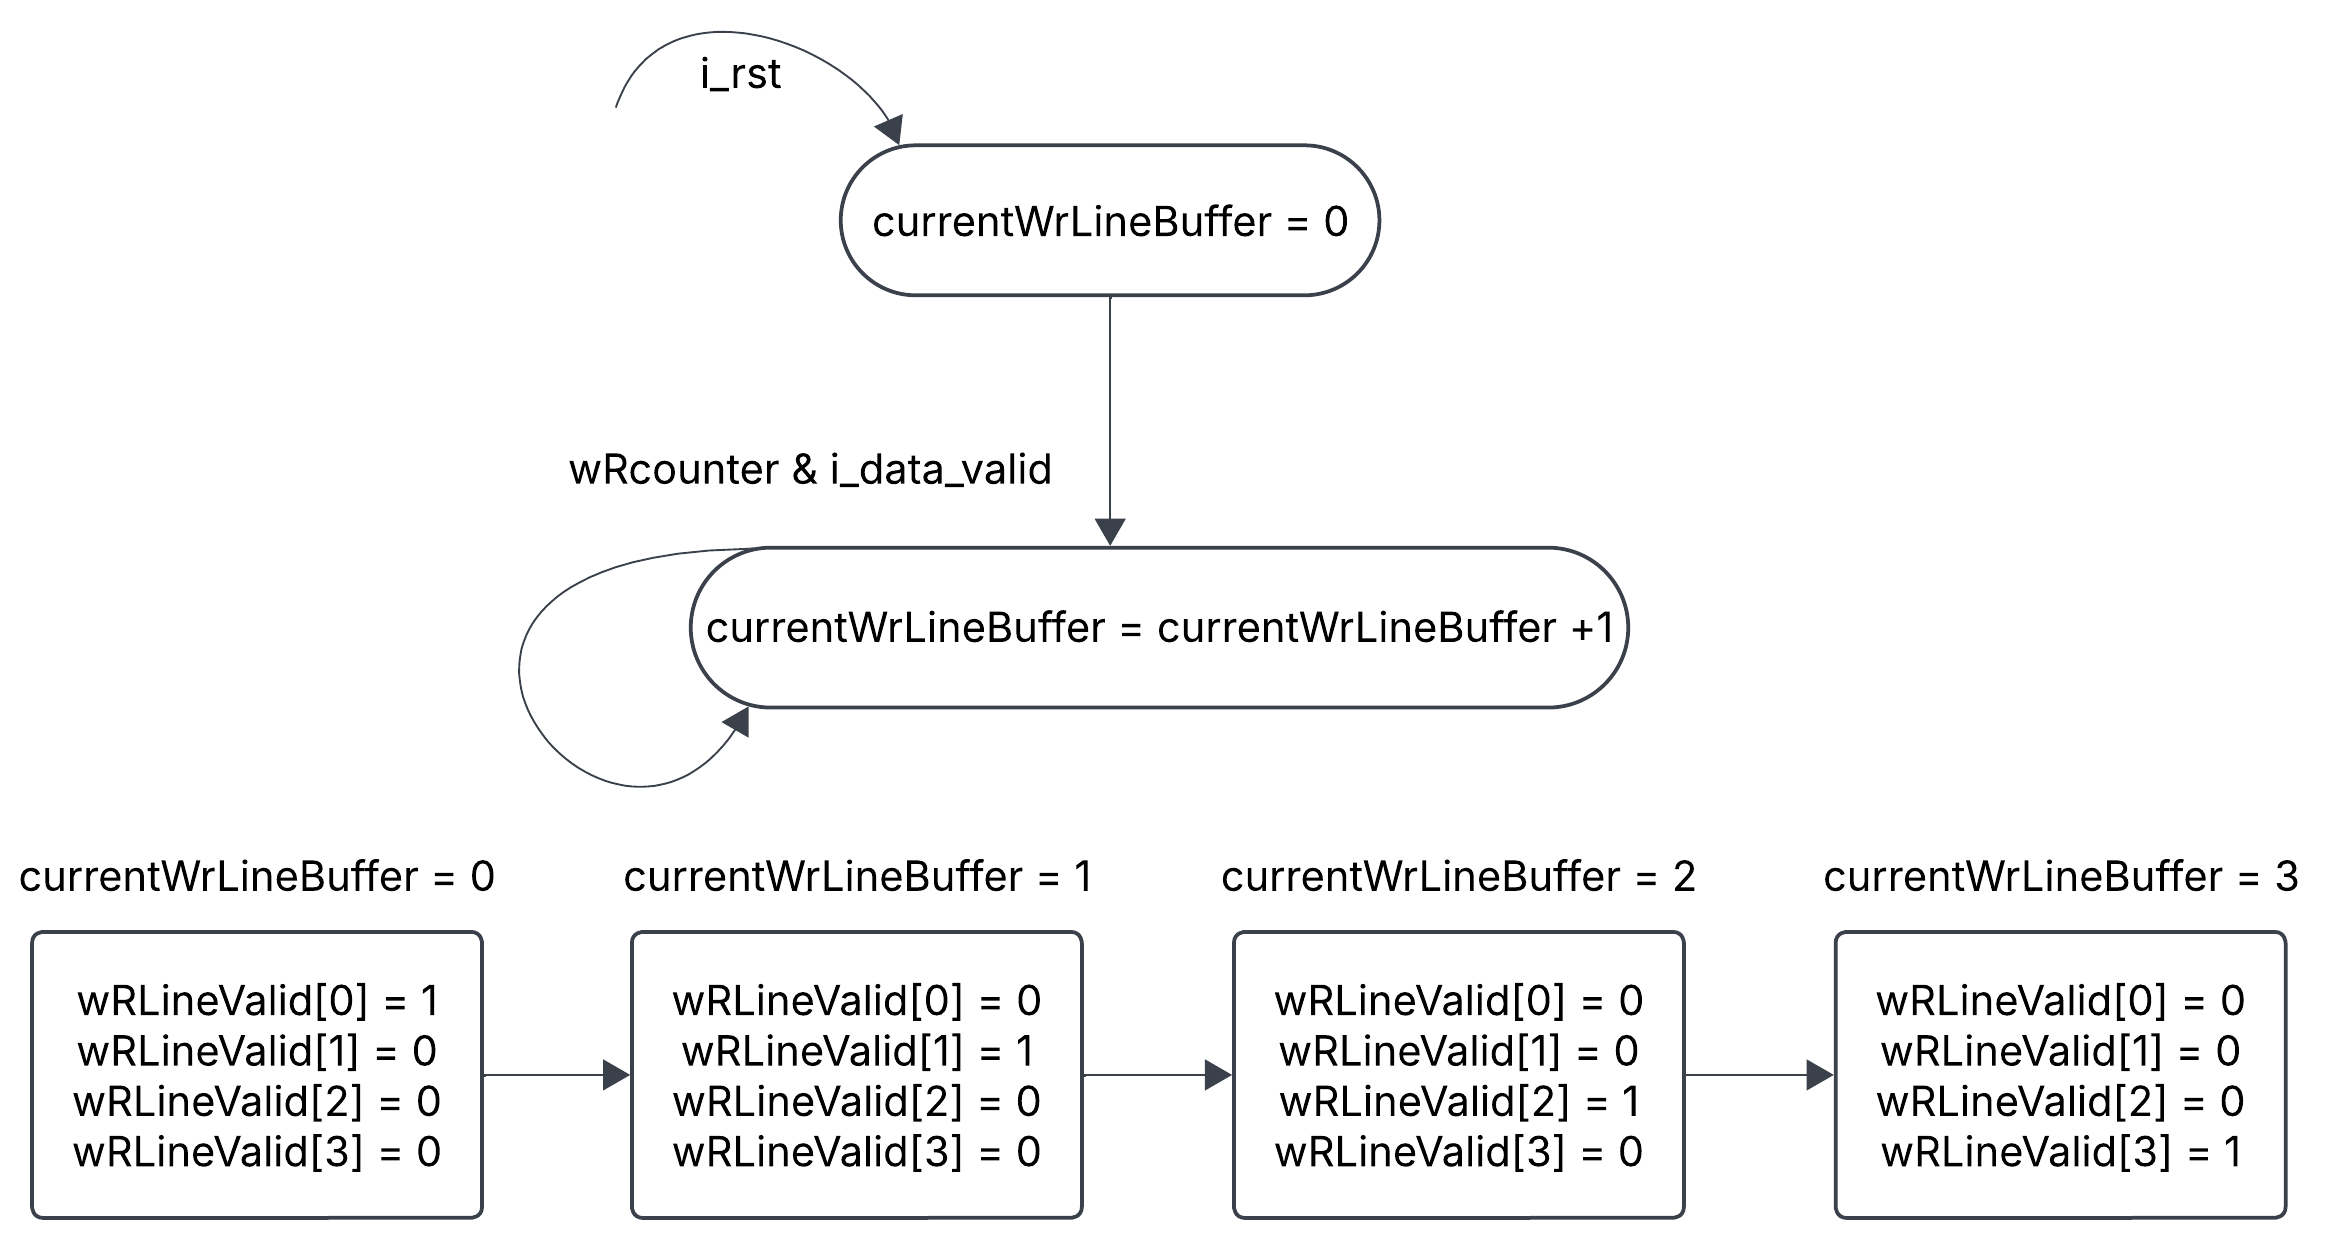
\includegraphics[width=0.75\linewidth]{images/convWrcontrol.png}
    \caption{Write Line Buffer counter and state diagram}
    \label{fig:wrBufferControl}
    \end{figure}

    \vspace{-1em}  % adjust this to control spacing

    \begin{figure}[H]
    \centering
    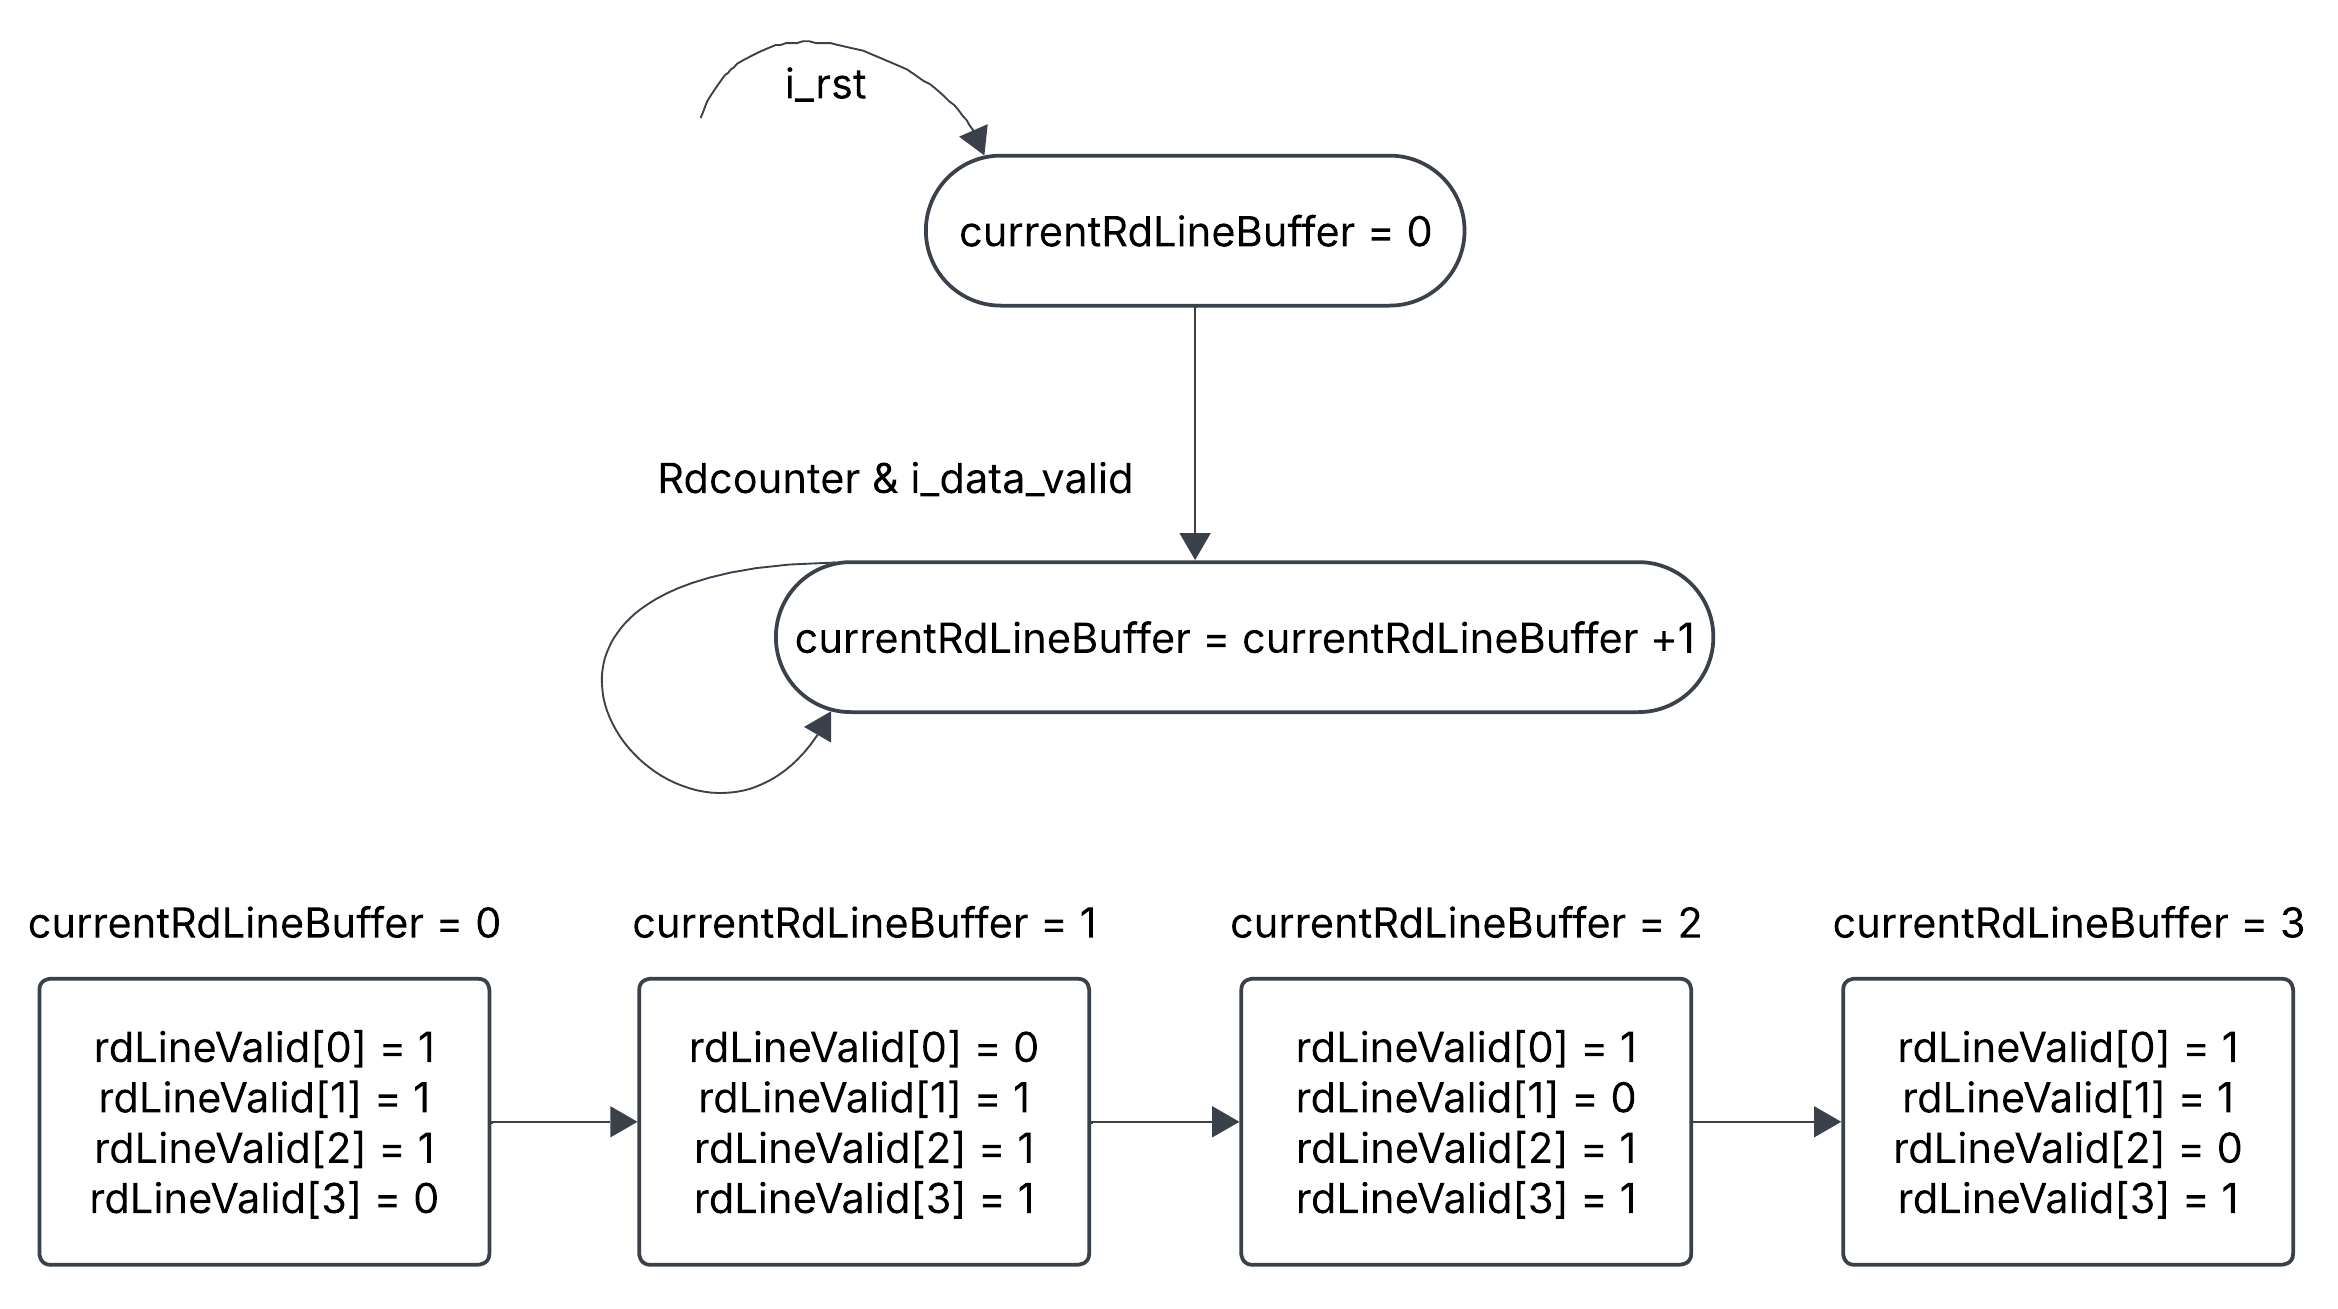
\includegraphics[width=0.75\linewidth]{images/convRdcontrol.png}
    \caption{Read Line Buffer counter and state diagram}
    \label{fig:rDBufferControl}
    \end{figure}


    \subsection{Maxpool Architecture}
    \noindent
    The figure \ref{fig:maxpool_operation} shows the maxpool operation, of how the kernel moves across the image, and is modelled in the same way at the hardware level. The maxpool and convolution logic are connected through the AXI  Stream. The output of the convolutional layer, which is input for the maxpool layer, is 24 bits wide, where the MSB bit represents the sign of the number and the integer bits are 11 bits wide, followed by 12 bits of fraction as shown in the figure \ref{fig:conv_result}. The integer part is increased from 3 to 10 bits to accommodate the product of image data and kernel as discussed in \ref{sec:conv_architecture}. 
    \par \noindent
    One of the critical parts while designing the maxpool control logic is taking into account the fact that maxpool processes the convolution data at a faster rate than it receives it from the convolution logic, which is because of the stride of 2. Thus, ensuring an appropriate set of pixels in synchronisation with the input convolved data became a challenging task.
    \par \noindent
    The maxpool layer uses 4 line buffers to store the data required for the convolution operation, as shown in the Figure \ref{fig:max_buff_arch} here, one line buffer stores convolution data row-wise.  The kernel in the maxpool layer is of 2x2, thus at a time, two line buffers are processed. Also, there is a stride of two, hence another two buffers store the data for the next processing. The ‘currentWrlinebuffer’ and ‘currentRdlinebuffer’ are the signals which control data being transferred to the maxpool data logic. Since the maxpool simply involves a comparison operation and no addition, multiplication, the result is of the same width as the convolution result.
    
     \begin{figure}[ht]
        \centering
        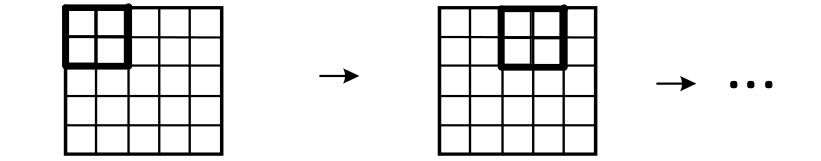
\includegraphics[width=0.75\linewidth]{images/maxpool.png}
        \caption{Maxpool Operation}
        \label{fig:maxpool_operation}
    \end{figure}
    
    \noindent The maxpool module, upon receiving the data from line buffers, computes the result for one 2x2 kernel in two stages as shown in Figure \ref{fig:stagewise_conv}. In the first stage, two pairs of data are compared with each other and the maximum of each respective pair is stored in an intermediate register, compIntm1 and compIntm2. The next stage computes the maximum of the maximum of two from the previous stage, which were stored in the intermediate registers.

    \begin{figure}[h!]
        \centering
        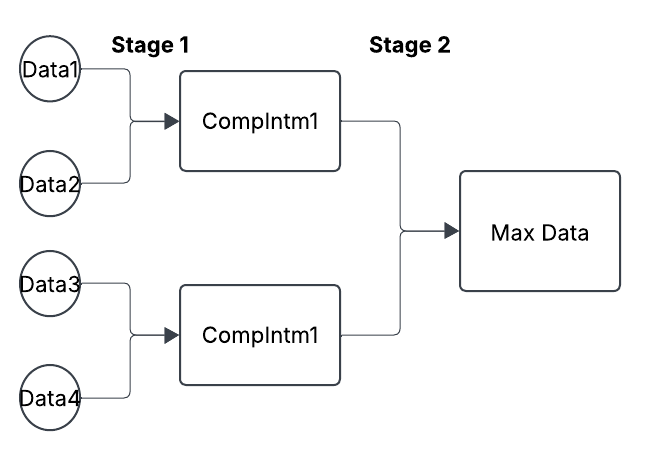
\includegraphics[width=0.75\linewidth]{images/stageWiseMax.png}
        \caption{Stagewise operation of Maxpool Layer}
        \label{fig:stagewise_conv}
    \end{figure}

    \begin{figure}[H]
        \centering
        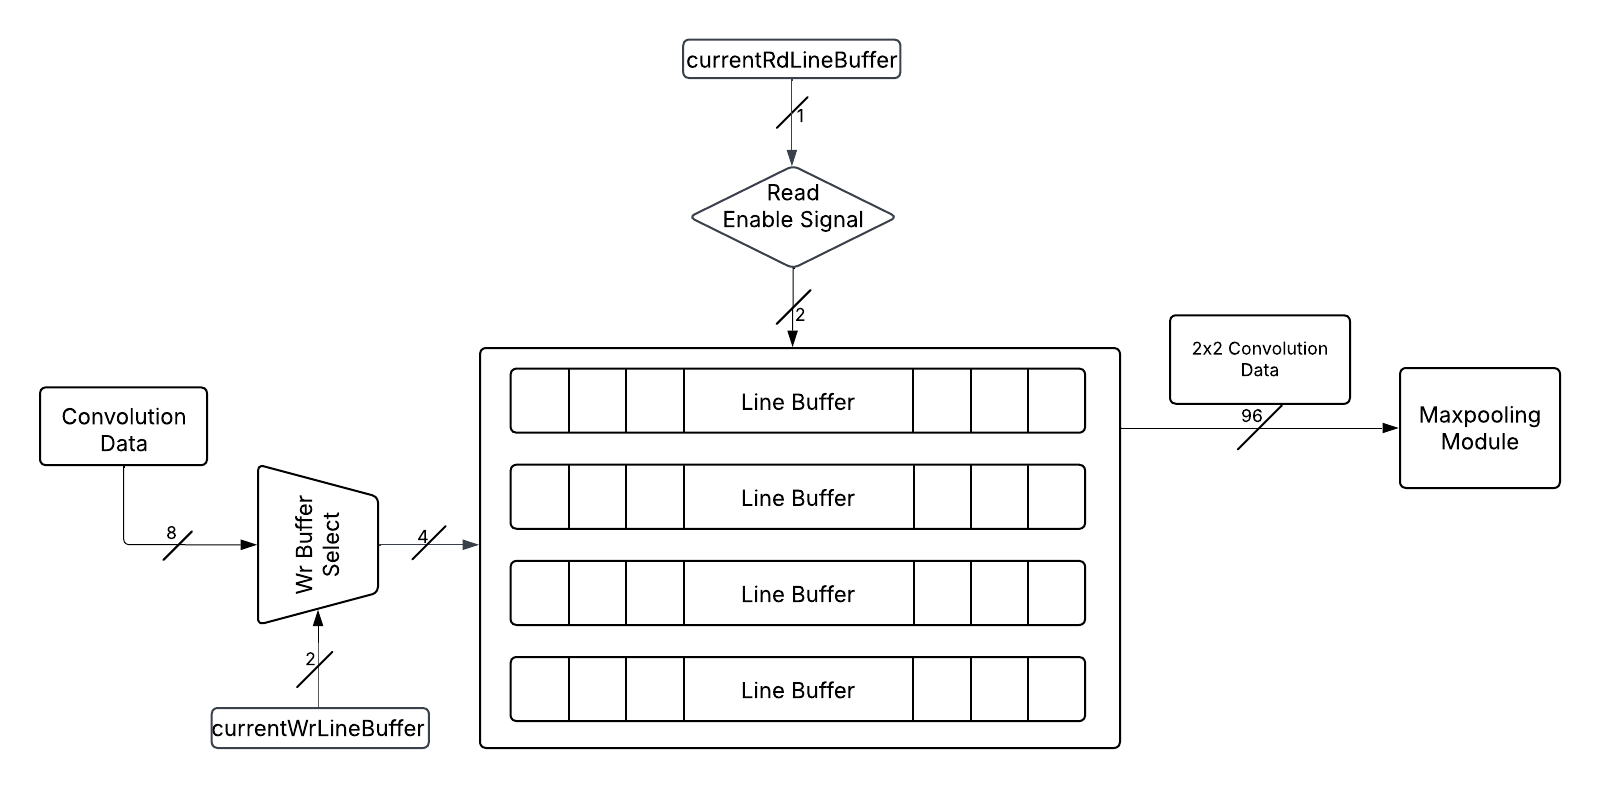
\includegraphics[width=\linewidth]{images/maxpool_architecture.png}
        \caption{Maxpool Buffer Architecture}
        \label{fig:max_buff_arch}
    \end{figure}
    
    \section{Overall Integration}
    \subsection{Convolution Maxpool Integration}
    \noindent
    Upon successful design and testing of the convolution and maxpool modules, they must be integrated for proper feature map generation. At the top level, both of the modules are designed around the AXI stream protocol interface, and thus are connected using the AXI stream interface. Since the fully connected layer is implemented at the PS level, the convolution and maxpool modules are combined to form a single AXI-based maxpooled data stream generating IP block. Figure \ref{fig:conv_max_integration} shows the interfacing between the convolution and maxpool module. It can be seen that all the signals, i.e. the ready, valid and data signals, are based on the AXI Stream protocol, the respective signals have been mapped to the appropriate ports according to the protocol.

    \begin{figure}[h]
        \centering
        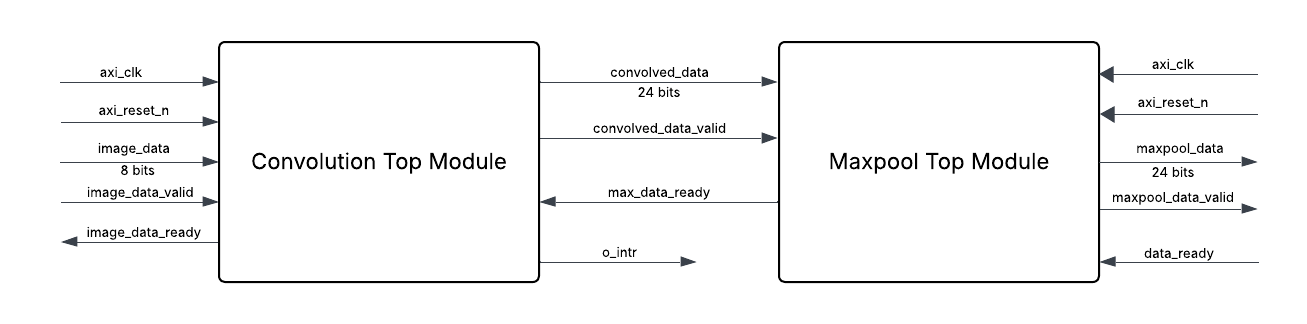
\includegraphics[width=1\linewidth]{images/conv_max_integration.png}
        \caption{Convolution Maxpool Integration}
        \label{fig:conv_max_integration}
    \end{figure}

    \subsection{Block Level Integration}
    \noindent
    After successful completion of design, integration and verification of the convolution and maxpool modules, the integrated design is packaged as a single IP using the Vivado IP Packager tool. This step is necessary to ensure that the convolution and maxpool as a whole design could be interfaced with the AXI DMA and the ZYNQ7 Processing System(PS). Creating the block design involves several steps, starting with configuring the IP repo to be able to use our packaged IP. In this stage majority of configurations are made, such as setting the Clock Frequency, PS UART baud rate, and enabling or disabling certain ports. The IP, which is created in this project, works on an AXI Stream protocol. DMA has an AXI\_LITE interface, using which it communicates with the PS. The interfacing between PS and the IP is enabled by the DMA, which connects to the IP through the AXI Stream MM2S and S2MM at the master port and slave port, respectively. As can be seen in the figure \ref{fig:convMaxBD}, an IP \textit{AXI Stream Data Width Converter} is used to interface master port of the IP and the slave port of the DMA, because the slave port of the master supports 32-bit data, and the output of the convolution is 24 bits wide.

    \begin{figure}[H]
        \centering
        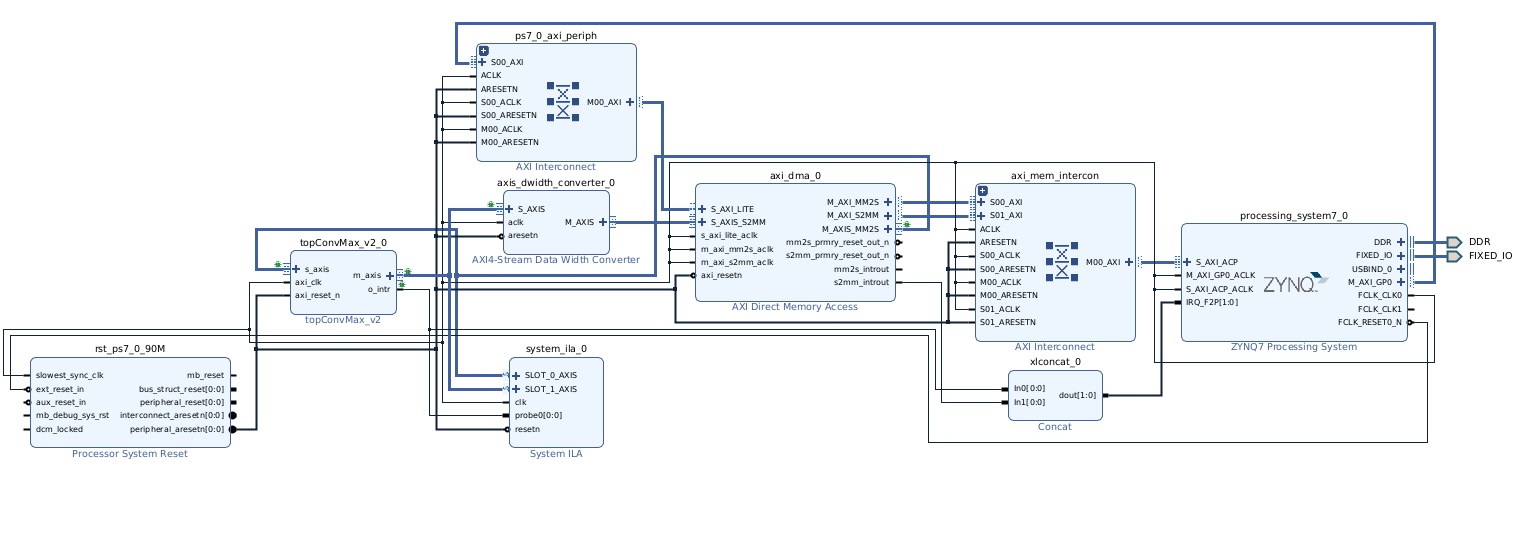
\includegraphics[width=1\linewidth]{images/convMaxBlockDesign.png}
        \caption{Convolution and Maxpool IP Block Design}
        \label{fig:convMaxBD}
    \end{figure}

    \noindent
    The following figure \ref{fig:addressMap} shows the address map for the memory-mapped interfaces. It can be verified from the address map that the appropriate ports are connected at the respective ports, and it also shows the addresses.

    \begin{figure}[H]
        \centering
        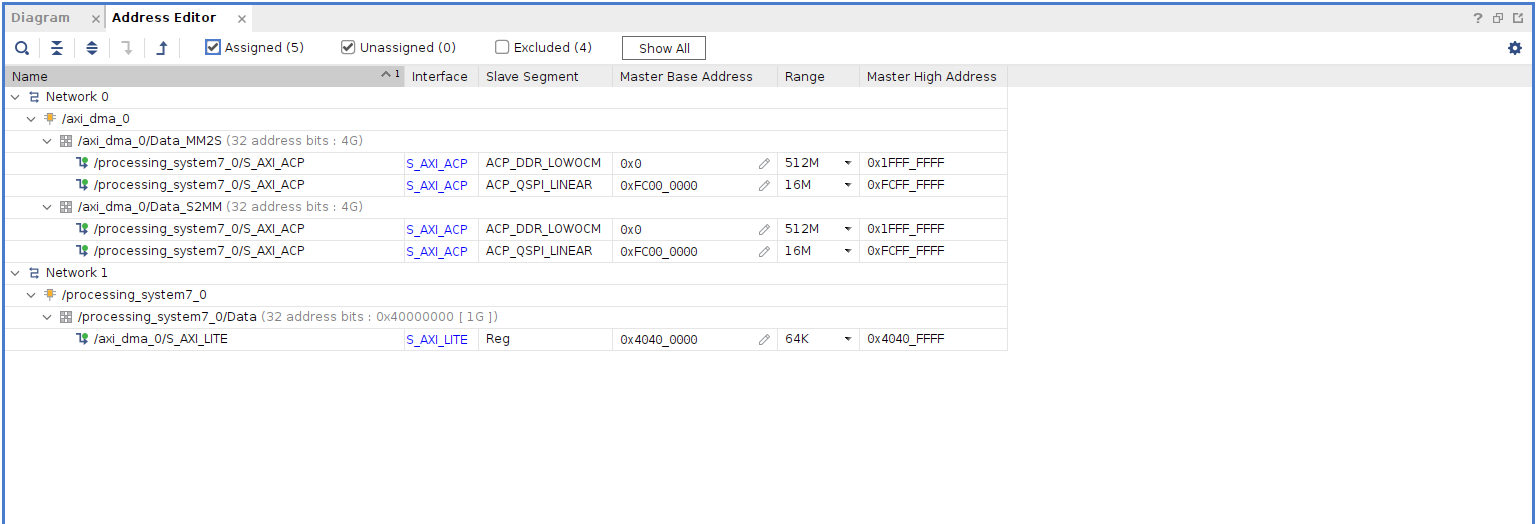
\includegraphics[width=1\linewidth]{images/addressMap.png}
        \caption{Address Map for memory-mapped interfaces}
        \label{fig:addressMap}
    \end{figure}
    \newpage
    